\documentclass[11pt]{article}

\usepackage[letterpaper,margin=1in]{geometry}
\usepackage[T1]{fontenc}
\usepackage[utf8]{inputenc}
\usepackage{palatino}
\usepackage{amsmath,amssymb,amsfonts,stmaryrd,mathtools}
\usepackage{amsthm}
\usepackage{array}
\usepackage{booktabs}
\newcolumntype{L}[1]{>{\raggedright\arraybackslash}p{#1}}
\usepackage{enumitem}
\usepackage{listings}
\usepackage{xcolor}
\usepackage{tikz}
\usepackage[protrusion=true,expansion=false]{microtype}
\usepackage[hidelinks]{hyperref}

\usetikzlibrary{arrows.meta,positioning,fit,backgrounds,calc}

\emergencystretch=2.5em

\theoremstyle{definition}
\newtheorem{definition}{Definition}[section]
\newtheorem{example}[definition]{Example}
\newtheorem{obligation}[definition]{Obligation}
\theoremstyle{plain}
\newtheorem{claim}[definition]{Claim}
\newtheorem{proposition}[definition]{Proposition}
\theoremstyle{remark}
\newtheorem{remark}[definition]{Remark}
\newtheorem{aside}[definition]{Aside}
\newtheorem{question}[definition]{Open question}

\newcommand{\rhoc}{\textsf{rho}}
\newcommand{\sem}[1]{\llbracket #1 \rrbracket}
\newcommand{\Proc}{\mathsf{Proc}}
\newcommand{\T}{\mathbb{T}}
\newcommand{\M}{\mathsf{M}}
\newcommand{\unit}{\mathsf{unit}}
\newcommand{\fmap}{\mathsf{map}}
\newcommand{\bind}{\mathsf{flatMap}}
\newcommand{\zero}{\mathsf{zero}}
\newcommand{\meas}{\mathsf{measure}}
\newcommand{\alg}{\mathsf{alg}}
\newcommand{\cost}{\mathsf{C}}
\newcommand{\hist}{\mathsf{H}}
\newcommand{\hyp}{\mathsf{Hyp}}
\newcommand{\lax}{\bigcirc}
\newcommand{\signed}[2]{\{#1\}_{#2}}
\newcommand{\fe}{\texttt{foreach}}
\newcommand{\gate}[2]{\texttt{\{\%}\,#1\,\texttt{\%\}[}#2\texttt{]}}

% Brand. The language is f1r3|@ng (spoken f1r3lang). `|' is parallel
% composition and `@' is quotation.
\newcommand{\flang}{\textsf{f1r3\textbar @ng}}
\newcommand{\flangbf}{\textsf{\bfseries f1r3\textbar @ng}}

\definecolor{kwcol}{rgb}{0.15,0.15,0.60}
\definecolor{strcol}{rgb}{0.55,0.18,0.12}
\definecolor{comcol}{rgb}{0.38,0.44,0.38}

\lstdefinestyle{code}{
  basicstyle=\ttfamily\footnotesize,
  keywordstyle=\color{kwcol}\bfseries,
  stringstyle=\color{strcol},
  commentstyle=\color{comcol}\itshape,
  showstringspaces=false,
  breaklines=true,
  columns=fullflexible,
  frame=leftline,
  framesep=6pt,
  xleftmargin=10pt,
  aboveskip=8pt,
  belowskip=8pt,
}

\lstdefinelanguage{rholang}{
  morekeywords={new,in,for,foreach,yield,match,contract,where,if,then,else},
  morecomment=[l]{//},
  morestring=[b]",
}

\lstdefinelanguage{mettail}{
  morekeywords={Module,Theory,theory,import,from,as,Types,Exports,Replacements,
    Terms,Equations,Rewrites,Monads,over,unit,flatMap,map,zero,measure,algebra,
    commutative,laws,Empty,free,let,in,if,then,subst},
  sensitive=true,
  morecomment=[l]{//},
  morestring=[b]",
}

\lstdefinelanguage{bnf}{
  morekeywords={foreach,yield,where},
  sensitive=true,
  morecomment=[l]{--},
  morestring=[b]",
}

\lstset{style=code,language=rholang}

\title{\bf Monadic Types and the \texttt{foreach} Comprehension\\ in \flangbf{}\\[2mm]
\large A synchronous comprehension over declared data monads,\\
\large with explicit cost}

\author{L.G. Meredith\\ \small F1R3FLY.io}
\date{October 2026 --- draft}

\begin{document}
\maketitle

\begin{abstract}
\noindent
\flang{} (spoken \emph{f1r3lang}; formerly MeTTaIL, and before that rholang~1.4)
has one comprehension, \texttt{for}, and it binds in the \emph{space}: its
sources are channels, its data are shared with concurrent writers, and when
several candidate matchings are available it resolves them by choosing one.
This note adds a second comprehension, \fe{}, which binds in a \emph{declared
data monad}: its sources are terms of a monadic sort, it meets no writer, and when
a nondeterministic monad presents several candidates it resolves them by
summing over all of them. The two comprehensions share a surface and a
vocabulary --- patterns, per-group \texttt{where} clauses, \texttt{;} for
sequence --- and differ in exactly the place where binding happens.

The design has three parts. In the data definition sublanguage, a
\texttt{Monads} builder declares that a sort is a monad and gives the
interpretation of \(\unit\), \(\bind\) and optionally \(\fmap\) as rewrites,
together with four optional capabilities --- a zero, commutativity, a measure,
and an algebra on processes --- each of which licenses a specific feature of
the comprehension. The monad laws are recorded as proof obligations, not as
equations, so that matching modulo a theory never meets higher-order
unification. In the control flow sublanguage, \fe{} is synchronous in a precise
sense: its binding skeleton is a burst of internal steps that no other
process can observe, so it may be treated as a single step and sequenced with
\texttt{;} exactly as the synchronous send of rholang~1.1 is. In the
cost-accounted surface, the comprehension carries two gates,
\gate{\texttt{foreach( p <- m ) yield} \gate{P}{t}}{s},
the outer funding every \emph{binding} and the inner funding every
\emph{body}. Per-binding charging turns the data-dependent cost of the
comprehension into an estimation problem: a linear funding proof needs a bound
on the measure of the monadic instance, and the note sets out where such
bounds come from.

Because \fe{} is a conservative extension of the core, it need not be
implemented by translation into \texttt{for}. The translation is retained as
the reference semantics, and a native implementation is correct when it is
\emph{gradedly} bisimilar to it --- the same behaviour and the same bill.
\end{abstract}

\tableofcontents

%=============================================================================
\section{Two comprehensions}
\label{sec:intro}

The comprehension is the shape data access takes when written down
honestly: name a source, filter it, project the survivors, act. SQL,
LINQ~\cite{LINQ}, XQuery's FLWOR and the list comprehension~\cite{Wadler87}
are the same shape, and Wadler's observation that the comprehension is
monadic~\cite{Wadler92}, in the sense Moggi gave to notions of
computation~\cite{Moggi91}, is what makes the family a family: every one of them
is a notation for \(\bind\) in some monad.

\flang{}'s receipt
\begin{lstlisting}
for( ptrn <- chan where cond ) P
\end{lstlisting}
is that shape with the \texttt{DO} made first-class~\cite{F1R3Dev}. But the
monad it binds in is unusual. The source is a channel; the datum is produced by
a concurrently running writer; the join \texttt{\&} is a rendezvous; the
communication rule substitutes the datum into the continuation and thereby
\emph{witnesses} the meeting. Call this the \emph{space} monad. Its bind is
asynchronous, it is shared, and it is nondeterministic in the strong sense that
competing readers race.

Developers also need the other kind of comprehension --- the one LINQ and
Scala's \texttt{for} provide over a collection already in hand. A term
received on a channel may itself be a list, a bag, a tree of findings, a
distribution. Walking it with \texttt{for} is possible only by first spilling
it onto a channel, which is both expensive and wrong: it exposes a private
traversal to every other reader of that channel, and it turns a deterministic
computation over a value into a race.

\fe{} is the missing comprehension. It binds in a \emph{data monad} declared
in the data definition sublanguage (DDL), and it is synchronous: the traversal
is invisible from outside, so the comprehension may be treated as one step.

\paragraph{Choose versus sum.} The cleanest way to see the difference is through
the word the developer document uses for the thread running through
\flang{}'s semantics: \emph{candidate}~\cite{F1R3Dev}. A candidate is one way
of assigning data to the patterns of a comprehension.
\begin{itemize}[nosep]
\item In \texttt{for}, candidates are resolved by \emph{choice}. One fires; the
others do not.
\item In \fe{} over a nondeterministic monad, candidates are resolved by
\emph{aggregation}. All of them fire, and \(\bind\) sums their contributions.
\end{itemize}
Figure~\ref{fig:choosesum} draws the distinction. Section~\ref{sec:graded}
shows that it is exactly the distinction the graded \texttt{where} clause needs.

\begin{figure}[t]
\centering
\resizebox{\linewidth}{!}{%
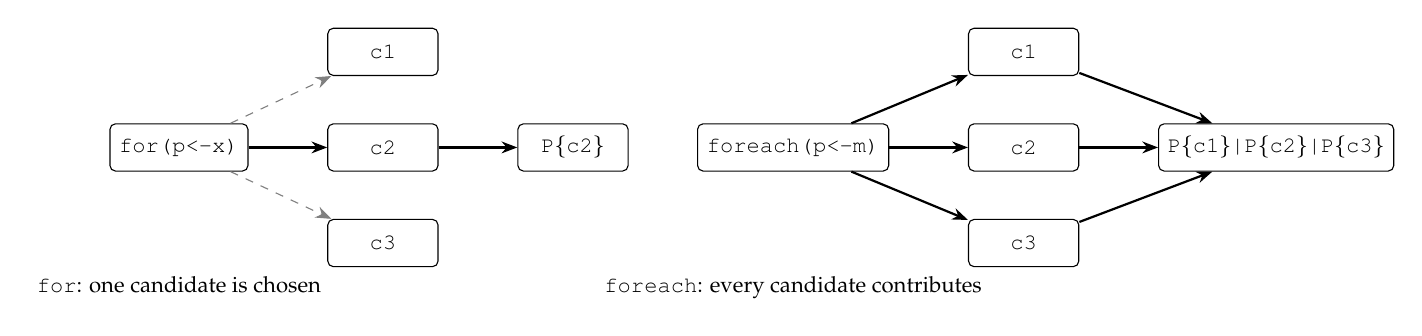
\begin{tikzpicture}[
  node distance=6mm and 10mm,
  box/.style={draw, rounded corners=2pt, minimum width=14mm, minimum height=6mm,
    font=\footnotesize\ttfamily},
  lab/.style={font=\footnotesize},
  >={Stealth[length=2mm]}]
  % left: for
  \node[box] (r) {for(p<-x)};
  \node[box, above right=of r] (c1) {c1};
  \node[box, right=of r] (c2) {c2};
  \node[box, below right=of r] (c3) {c3};
  \draw[->, thick] (r) -- (c2);
  \draw[->, dashed, gray] (r) -- (c1);
  \draw[->, dashed, gray] (r) -- (c3);
  \node[box, right=of c2] (k1) {P\{c2\}};
  \draw[->, thick] (c2) -- (k1);
  \node[lab, below=12mm of r] {\texttt{for}: one candidate is chosen};
  % right: foreach
  \begin{scope}[xshift=78mm]
  \node[box] (m) {foreach(p<-m)};
  \node[box, above right=of m] (d1) {c1};
  \node[box, right=of m] (d2) {c2};
  \node[box, below right=of m] (d3) {c3};
  \foreach \d in {d1,d2,d3} \draw[->, thick] (m) -- (\d);
  \node[box, right=of d2, minimum width=22mm] (k2) {P\{c1\}|P\{c2\}|P\{c3\}};
  \foreach \d in {d1,d2,d3} \draw[->, thick] (\d) -- (k2);
  \node[lab, below=12mm of m] {\fe{}: every candidate contributes};
  \end{scope}
\end{tikzpicture}}
\caption{The two resolution disciplines for candidates. Over a bag, the
aggregate on the right is literally a parallel composition, because
\texttt{PPar} is a bag (\S\ref{sec:algebra}).}
\label{fig:choosesum}
\end{figure}

\paragraph{Contributions.}
\begin{enumerate}[nosep]
\item A \texttt{Monads} builder for the DDL, with the laws as obligations and
four capabilities (zero, commutativity, measure, algebra on processes) each
tied to one feature of the comprehension (\S\ref{sec:ddl}).
\item The \fe{} comprehension: its syntax, static discipline, reference
semantics and a precise criterion for synchrony (\S\ref{sec:cfl}).
\item Sequencing with \texttt{;}, extending rholang~1.1's synchronous send
sugar, together with a sequenceable fragment of bodies that recovers a genuine
completion barrier where one is meaningful (\S\ref{sec:seq}).
\item An explicit cost-accounted surface with two gates, per-binding charging,
an atomic $n$-ary outer gate, and a precharge discipline for linear funding
proofs (\S\ref{sec:cost}).
\item An implementation stance --- native evaluation, the translation retained
as specification, graded bisimulation as the correctness criterion --- and a
map of what changes in the node (\S\ref{sec:impl}).
\item An account of the interaction with every other feature of \flang{}
(\S\ref{sec:interactions}), and a first tranche (\S\ref{sec:tranche}).
\end{enumerate}

%=============================================================================
\section{Background}
\label{sec:background}

This section fixes the parts of \flang{} the feature touches. Fuller
treatments are in the developer document~\cite{F1R3Dev} and the GSLT
reference~\cite{GSLTintro}.

\flang{} is built on the reflective higher-order \rhoc{}
calculus~\cite{MR05}, presented in its own DDL as one theory among others.

\subsection{The data definition sublanguage}

A language definition is a \texttt{Theory}. Its body is an ordered chain of
postfix builders --- \texttt{Types}, \texttt{Exports}, \texttt{Replacements},
\texttt{Terms}, \texttt{Equations}, \texttt{Rewrites} --- applied to a starting
theory, and theories combine by join, meet and difference over shared ancestors
\cite{modulesyntax}. Every element introduced by a builder carries an origin
token, and two elements are identified exactly when their origins agree; this is
what makes a join a pushout rather than a union, and what produces the
\texttt{[join-collision]} and \texttt{[unshared-name]} diagnostics.

Term constructors are written in judgement form,
\begin{lstlisting}[language=mettail]
PInput . n:Name, ^x.p:[Name -> Proc] |- n "?" x "." "{" p "}" : Proc;
PPar   . ps:HashBag(Proc) |- "{" ps.*sep("|") "}" : Proc;
\end{lstlisting}
with binders \verb|^x.p| as first-class arguments, and three built-in
collection sorts \texttt{HashBag}, \texttt{Set} and \texttt{List} over a
category. There are no user-declared sort constructors: in the reference
elaborator a sort is either a category or a built-in collection of one. That
fact governs the first tranche of this design.

\subsection{The control flow sublanguage}

The comprehension has the form
\begin{lstlisting}
for( ptrn_11 <- chan_11 & ... & ptrn_1n <- chan_1n  where cond_1 ;
     ...                                                         ;
     ptrn_k1 <- chan_k1 & ... & ptrn_km <- chan_km  where cond_k ) P
\end{lstlisting}
with \texttt{\&} for simultaneity within a group, \texttt{;} for sequence
between groups, and a \texttt{where} per group that may mention any variable
bound in that group or an earlier one. Three arrows distinguish a consuming
read \texttt{<-}, a persistent read \texttt{<=} and a peek \texttt{<<-}. A
failed guard leaves the datum in the space: a failed transaction is not rolled
back, it never began~\cite{F1R3Dev}.

Rholang~1.1 also provides a synchronous send, \verb|x!?(Q); K|, which the
node's normaliser desugars as
\begin{lstlisting}
new r in { x!(*r, Q) | for( _ <- r ){ K } }
\end{lstlisting}
so that \texttt{K} runs once the receiver on \texttt{x} acknowledges on the
fresh name \texttt{r}~\cite{f1r3nodeOTE}. Chains
\verb|x1!?(Q1); ...; xn!?(Qn); K| are nested instances.

\subsection{The cost-accounted surface}

Cost accounting is written in the language rather than bolted onto an
interpreter~\cite{CostRho}. A signed term \(\signed{P}{s}\), concretely
\verb|{% P %}[s]|, runs \texttt{P} once a token for signature \texttt{s} is
available; a budget is a stack \verb|s :: s :: ... :: ()| whose depth is the
number of operations it funds. Signatures are ground names, sections
\verb|# P|, and compounds. The surface already admits per-clause signed binds,
\begin{lstlisting}
{% for( {% y1 <- x1 %}[s1] & {% y2 <- x2 %}[s2] ) P %}[ s0 ]
\end{lstlisting}
in which each rendezvous surface is funded independently, and in the native
four-sort grammar the continuation slots of \texttt{for} and send have the
signed-term sort \(\T\). That sorting --- \emph{wrapping by construction} ---
is what makes subject reduction coincide with the absence of unmetered
execution~\cite{CostMonad}.

\subsection{Monads one level up}

The GSLT reference treats three monads: the cost monad \(\cost\), the history
monad \(\hist\) and the Hypercube construction \(\hyp\)~\cite{GSLTintro,
CostMonad, History, Hypercube}. All three are endofunctors on the category of
theories: they take a theory and return a metered, logged or typed theory.

The monads of this note live one level down. A declaration
``\(\M\) is a monad'' is a statement \emph{inside} a theory, about one of its
sorts. The distinction matters in two places. In prose, the phrase ``the
monad'' becomes ambiguous; this note says \emph{data monad} for the new kind and
\emph{theory-level monad} for \(\cost\), \(\hist\) and \(\hyp\). And in
semantics, the theory-level monads act on theories that contain data monads,
which raises the question of whether the declaration survives them.

\begin{proposition}[Laws modulo erasure]
\label{prop:modulo-erasure}
Let theory \(T\) declare a data monad \(\M\) whose laws hold in \(T\). Then
\(\cost(T)\) and \(\hist(T)\) carry the declaration, and the laws hold in each
up to the corresponding erasure back to \(T\), but not in general on the nose.
\end{proposition}

\begin{proof}[Sketch]
The two sides of the left unit law,
\(\bind(\unit(a), k)\) and \(k\,a\), differ by one application of the
\(\bind\) rewrite. In \(\cost(T)\) that application is gated and consumes a
token; in \(\hist(T)\) it is logged as an event. The two sides therefore differ
in cost and in history, and agree after the erasures \(\cost(T)\to T\) and
\(\hist(T)\to T\) studied in~\cite{TwoErasures}. The right unit and
associativity laws are similar.
\end{proof}

This is the expected behaviour, not a defect, and it anticipates the
correctness criterion of \S\ref{sec:impl}: once cost is explicit, ``the same
computation'' means the same behaviour \emph{and} the same bill.

%=============================================================================
\section{Declaring a data monad}
\label{sec:ddl}

\subsection{The prerequisite: a sort constructor}

A monad is a sort constructor \(\M(-)\) with structure. \(\fmap\) alone needs
two element sorts, \((A \to B) \to \M(A) \to \M(B)\). The DDL has no
user-declared sort constructors, so the design proceeds in two steps.

\paragraph{Step 1: the built-in collections.} \texttt{List}, \texttt{Set} and
\texttt{HashBag} are already sort constructors, and they are the canonical
monads: the list monad, the finite powerset monad, and the finite multiset
monad. Declaring them monadic needs no new sort machinery. They are declared once,
in a prelude supplied by the toolchain, and are available to every theory.

\paragraph{Step 2: sort parameters.} The general feature extends
\texttt{Types} with parameterised categories,
\begin{lstlisting}[language=mettail]
Types { Tree(A); }
\end{lstlisting}
where \texttt{A} ranges over categories. This is the real feature, and it is
independently useful: the Hypercube construction currently generates type
systems over unparameterised sorts~\cite{Hypercube}.

\paragraph{A rejected alternative.} A theory parameter can stand in for a type
parameter --- \texttt{Theory List(e: EmptySet)} is a list of whatever
\texttt{e} exports. But then \(\M\) is a map from theories to theories, the
feature climbs back to the level of \(\cost\) and \(\hist\), and the sharing
discipline objects: \texttt{List(List(s))} reintroduces the list constructors
along its own chain and draws \texttt{[repeat-label]}. The diagnostic is
correct, and the alternative is rejected.

\subsection{The \texttt{Monads} builder}

A new postfix builder declares one or more data monads. Its entries name the
monad, the sort it is a monad on, the interpretation of the operations, and
the capabilities it claims. The following is the prelude declaration of the
list monad, written with a sort variable \texttt{A} that Step~2 makes
available to users and that the prelude is permitted to use from the start.

\begin{lstlisting}[language=mettail]
Monads {
  Seq over List {
    unit    : (a)                    ~> [a];
    flatMap : ([], ^x.k)             ~> [];
    flatMap : ([a, ...r], ^x.k)      ~> (Concat (subst ^x.k a) (flatMap r ^x.k));
    zero    : [];
    measure : Length;
    algebra : Proc by seq;
    laws    : LeftUnit, RightUnit, Assoc;
  }
  Bag over HashBag {
    unit    : (a)                    ~> {a};
    flatMap : ({}, ^x.k)             ~> {};
    flatMap : ({a, ...r}, ^x.k)      ~> (Union (subst ^x.k a) (flatMap r ^x.k));
    zero    : {};
    commutative;
    measure : Size;
    algebra : Proc by PPar;
    laws    : LeftUnit, RightUnit, Assoc, Comm;
  }
}
\end{lstlisting}

The surface is illustrative; its content is not. Five decisions are embedded
in it.

\paragraph{The interpretation is a set of rewrites.} The DDL defines
operations only through rules, so \(\unit\) and \(\bind\) are given by cases
over the sort's constructors, with the continuation as a first-class
abstraction \verb|^x.k| of sort \verb|[A -> M(B)]|. These are ordinary
rewrites: they are oriented, they fire, and they ``wiggle'' like any other
rule of the theory. \(\fmap\) may be given explicitly for efficiency; when it
is, \(\fmap\,f = \bind(-, \unit\circ f)\) becomes one more obligation.

\paragraph{The laws are obligations, not equations.} Matching in \flang{} is
matching modulo the equations of the theory that types the channel. Placing
\(\bind(m, \lambda x.\unit(x)) = m\) in an \texttt{Equations} block would put
the matcher into higher-order unification, which is undecidable in general.
The \texttt{laws} entry therefore \emph{names} the laws; the elaborator records
them as obligations, discharged by proof (as the cost monad's laws are, in
Rocq and Lean) or by bounded exhaustive checking (as in the Sage harness), and
never hands them to the matcher.

\begin{obligation}[Monad laws]
For every declared data monad, the left unit, right unit and associativity
laws hold up to the equations of the theory.
\end{obligation}

\begin{obligation}[Confluence with the host theory]
\label{obl:confluence}
The \(\bind\) rewrites have no critical pair with the other rewrites of the
theory, modulo its equations, that fails to join.
\end{obligation}

Obligation~\ref{obl:confluence} is the one that makes \fe{} deterministic, and
\S\ref{sec:sync} explains why that is essential.

\paragraph{Capabilities are claims, and each one licenses a feature.} The four
optional entries are not decoration. Each corresponds to one feature of the
comprehension, and the elaborator refuses the feature where the capability is
absent.

\begin{center}
\small
\begin{tabular}{@{}L{0.17\textwidth}L{0.33\textwidth}L{0.40\textwidth}@{}}
\toprule
\textbf{Capability} & \textbf{Meaning} & \textbf{Licenses} \\
\midrule
\texttt{zero} & a unit for the monad's sum (MonadPlus) &
a crisp \texttt{where} clause inside \fe{} (\S\ref{sec:where}) \\[3pt]
\texttt{commutative} & order of independent binds is immaterial~\cite{Kock70} &
the join \texttt{\&} inside \fe{} (\S\ref{sec:groups}) \\[3pt]
\texttt{measure} & the number of times \(\bind(m,k)\) invokes \(k\) &
precharge for a linear funding proof (\S\ref{sec:precharge}) \\[3pt]
\texttt{algebra} & a map \(\M(\Proc) \to \Proc\) &
a \texttt{yield} whose body is a process (\S\ref{sec:algebra}) \\
\bottomrule
\end{tabular}
\end{center}

\noindent
Each capability carries its own obligation: commutativity is a law; the
measure must be exact (\S\ref{sec:precharge}); the algebra must satisfy the
Eilenberg--Moore laws~\cite{EilenbergMoore65}.

\paragraph{One sort may carry several monads.} The monads are named
(\texttt{Seq}, \texttt{Bag}) because a sort can legitimately carry more than
one monad structure, just as a rig carries two monoids on one carrier. A
comprehension may name the monad it binds in, \texttt{foreach[Seq](...)};
the qualifier may be omitted when exactly one monad is declared on the
source's sort.

\subsection{Monads and the algebra of theories}
\label{sec:modules}

A \texttt{Monads} entry is an element like any other, so it receives an origin
token at introduction and is carried through inheritance.

\begin{itemize}[nosep]
\item \textbf{Join.} Two theories that inherit \texttt{Seq} from one shared
instance join cleanly, and the comprehension sees one monad. Two theories that
independently declare a monad under the same name on the same sort draw
\texttt{[join-collision]}: they are two structures with one spelling.
\item \textbf{Difference.} Subtracting a constructor that a monad's rules
mention leaves the declaration dangling. That is a new diagnostic,
\texttt{[dangling-monad]}, and it is the analogue of the existing
\texttt{[forward-reference]}.
\item \textbf{Ordering.} A \texttt{Monads} block must follow the \texttt{Terms}
blocks whose labels its rules mention, by the existing chain discipline.
\item \textbf{Replacements.} Renaming a constructor preserves its identity and
therefore preserves the monad. Replacing a constructor by one of different arity
reproduces the open arity-drift problem already recorded for \texttt{PPar}:
the inherited \(\bind\) rules are written over a shape that no longer exists.
Whatever resolution is adopted there --- arity-preserving replacements, or a way
to declare inherited rules structural --- must be adopted here as well.
\item \textbf{Parameters.} Once Step~2 lands, monad transformers are theories
that take a monad as a parameter. This is the fourth rung of the DDL doing what
it was built for.
\end{itemize}

%=============================================================================
\section{The \texttt{foreach} comprehension}
\label{sec:cfl}

\subsection{Syntax}

\begin{lstlisting}[language=bnf]
Proc     ::= ... | Foreach | Foreach ";" Proc
Foreach  ::= "foreach" Qual? "(" Groups ")" "yield" Body
Qual     ::= "[" MonadName "]"
Groups   ::= Group ( ";" Group )*
Group    ::= Bind ( "&" Bind )* ( "where" Cond )?
Bind     ::= Pattern "<-" Term          -- Term of a monadic sort
Body     ::= "{" Proc "}"
\end{lstlisting}

The surface is chosen to coincide with \texttt{for} wherever the meanings
coincide, and to diverge visibly where they do not. Its cost-accounted form is
the subject of \S\ref{sec:cost}; until then, gates are elided.

\subsection{Static discipline}
\label{sec:static}

\paragraph{Sources are terms of a monadic sort.} In \texttt{for}, a source is a
channel. In \fe{}, a source is a term whose sort carries a declared monad. A
channel may not appear as a \fe{} source, because a receipt can block forever
and would break synchrony; a monadic term may not appear as a \texttt{for}
source except by being quoted into a name, in which case it is a channel and
nothing more. The two comprehensions nest freely in each other's bodies.

This places a requirement on the CFL that it has not had before: the sort of
the source expression must be known. Today \flang{} patterns match untyped.
\fe{} needs either sort inference for the source --- from the pattern that
bound it, from the theory that types the channel it arrived on --- or an
explicit qualifier.

\paragraph{One arrow.} Only \texttt{<-} is meaningful. Persistence \texttt{<=}
has no meaning over a value, and a peek \texttt{<<-} is moot because a term
source is never consumed. Both are refused rather than reinterpreted.

\paragraph{Typing.} Writing \(\Gamma\) for the bindings in scope,
\[
\frac{
\Gamma \vdash m : \M(A) \qquad
p : A \leadsto \Delta \qquad
\Gamma,\Delta \vdash c\ \textsf{cond} \qquad
\Gamma,\Delta \vdash P : \Proc
}{
\Gamma \vdash \texttt{foreach[}\M\texttt{]( } p \leftarrow m \texttt{ where } c \texttt{ ) yield \{ } P \texttt{ \}} : \Proc
}
\quad
\begin{array}{l}
\M\ \text{has an algebra on}\ \Proc\\
c \neq \texttt{true} \Rightarrow \M\ \text{has}\ \zero
\end{array}
\]
with the evident extension to several groups (each group's \(\Delta\) is in
scope for every later group) and to \texttt{\&} (which additionally requires
\(\M\) commutative).

\subsection{Groups: \texttt{;} and \texttt{\&}}
\label{sec:groups}

Between groups, \texttt{;} is dependent bind: in
\begin{lstlisting}
foreach( x <- m ; y <- n(x) ) yield { P }
\end{lstlisting}
the source of the second group may mention \texttt{x}, and the comprehension
means
\[
\bind\big(m,\ \lambda x.\,\bind(n(x),\ \lambda y.\,\unit(P))\big).
\]
The per-group scoping of \texttt{where} carries over unchanged.

Within a group, \texttt{\&} means \emph{independent} binds: neither source
mentions the other's variables. Its meaning is order-independent only if the
monad is commutative,
\[
\bind\big(m,\ \lambda x.\,\bind(n,\ \lambda y.\,k)\big) \;=\;
\bind\big(n,\ \lambda y.\,\bind(m,\ \lambda x.\,k)\big),
\]
and so \texttt{\&} is permitted
only on monads that claim \texttt{commutative}: \texttt{Bag} and the finite
powerset yes, \texttt{Seq} no. Without the restriction, \texttt{\&} over a list
would silently mean ``left, then right,'' and the symbol would mean
simultaneity in \texttt{for} and sequence in \fe{}.

\subsection{\texttt{where} in \texttt{foreach}}
\label{sec:where}

A crisp \texttt{where} clause inside \fe{} is a filter, and a filter needs
somewhere to send the candidates it rejects: the monad's zero. For a monad
without \texttt{zero}, a \texttt{where} clause in \fe{} is an elaboration error,
\texttt{[monad-no-zero]}.

The same keyword now has two operational readings, and the developer
document should state both:
\begin{itemize}[nosep]
\item in \texttt{for}, a failed guard \emph{leaves the datum in the space};
\item in \fe{}, a failed guard \emph{drops the binding}.
\end{itemize}
What reconciles them is that in both cases the rejected candidate is a
non-event. Nothing is consumed, nothing is undone, and nothing downstream sees
it.

\subsection{\texttt{yield}, and the algebra on processes}
\label{sec:algebra}

The body of a \fe{} is a process, so the comprehension produces a value of sort
\(\M(\Proc)\): a monadic collection of instantiated bodies. Something must turn
that value into a running process. Categorically, that something is an
Eilenberg--Moore algebra \(\alg : \M(\Proc) \to \Proc\)~\cite{EilenbergMoore65}.

\begin{itemize}[nosep]
\item For \texttt{Bag}, the algebra is free. \texttt{PPar} \emph{is} a
\texttt{HashBag(Proc)}, so yielding over a bag produces a parallel composition,
and the right-hand panel of Figure~\ref{fig:choosesum} is literal.
\item For \texttt{Seq}, there are two algebras. One forgets the order and
composes in parallel. The other composes in sequence, and exists only when the
bodies are sequenceable (\S\ref{sec:seq}). The prelude declares the
sequential one, and falls back to the parallel one with a warning when the
bodies are not sequenceable.
\item For a user-declared monad, a process-valued \texttt{yield} requires an
\texttt{algebra} entry; without one the elaborator reports
\texttt{[monad-no-algebra]}. A value-valued \texttt{yield}, producing an
\(\M(B)\) term rather than a process, does not need one, and is discussed with
sequencing.
\end{itemize}

\subsection{Reference semantics}
\label{sec:refsem}

The semantics of \fe{} is given by a translation into the core, which serves as
the specification against which any implementation is judged
(\S\ref{sec:impl}). For a single group over a built-in collection, the
translation walks the collection with a private recursive process. Each step
consumes one element, matches it, evaluates the guard, and either adds the
instantiated body to the accumulator or does not:
\begin{lstlisting}
new walk, done in {
  walk!( m, Empty ) |
  contract walk( @rest, @acc ) = {
    match rest {
      []         => done!( acc )
      [a, ...r]  => match a {
                      p where c => walk!( r, Add(acc, P) )
                      _         => walk!( r, acc )
                    }
    }
  } |
  for( @acc <- done ){ Alg(acc) }
}
\end{lstlisting}
\texttt{walk} and \texttt{done} are fresh, \texttt{Add} and \texttt{Empty} are
the monad's sum and zero, and \texttt{Alg} releases the accumulated bodies via
the algebra. For a user-declared monad the walk is replaced by the monad's own
\(\bind\) rules, with the continuation invoking the same match-and-guard step.
Dependent groups nest the walk.

The translation was designed so that \emph{each binding costs exactly one
communication on a private name}: one send on \texttt{walk} per element.
Entry and exit --- the first send on \texttt{walk} and the send on
\texttt{done} --- cost two more, a constant per comprehension. The reference
translation treats those two as administrative, funded by the cost-free unit
in the way the internalisation retraction of the cost monad treats its
administrative step~\cite{CostMonad}, so its metered count is exactly one per
binding. That choice is deliberate and is what makes per-binding charging
(\S\ref{sec:cost}) coincide with the reference translation's own count.

\subsection{Synchrony}
\label{sec:sync}

``Synchronous'' admits three readings, and only one is both meaningful and
achievable.

\begin{center}
\small
\begin{tabular}{@{}L{0.22\textwidth}L{0.38\textwidth}L{0.30\textwidth}@{}}
\toprule
\textbf{Reading} & \textbf{Meaning} & \textbf{Assessment} \\
\midrule
Data dependency & bindings precede the body &
too weak; \texttt{for} already has it \\[3pt]
Completion barrier & a continuation waits for every body to finish &
impossible in general; bodies spawn arbitrary processes \\[3pt]
Atomic skeleton & the binding skeleton resolves without observable
interleaving, then the bodies are released together &
adopted \\
\bottomrule
\end{tabular}
\end{center}

The atomic-skeleton reading has a precise formulation. In the reference
translation, every communication of the skeleton is on a name bound by the
translation's own \texttt{new}. Such communications are internal steps:
nothing outside the comprehension can participate in them.

\begin{proposition}[Synchrony]
\label{prop:sync}
Suppose the internal reduction of a \fe{} skeleton is confluent and
terminating. Then the translation of
\verb|foreach( p <- m where c ) yield { P }| is weakly bisimilar to a process
that performs no visible action until it becomes \(\alg\) applied to the
instantiated bodies.
\end{proposition}

\begin{proof}[Sketch]
All skeleton steps are communications on names restricted by the translation,
hence internal. Termination bounds the burst; confluence makes its end-point
unique up to structural congruence. A sequence of internal steps with a unique
end-point is absorbed by weak bisimulation.
\end{proof}

So \fe{} is synchronous exactly when its skeleton is a deterministic,
terminating burst of internal steps. The two hypotheses have different sources.
Termination is supplied by cost accounting: a funded skeleton is a bounded one
(\S\ref{sec:cost}). Confluence is Obligation~\ref{obl:confluence}, which is why
that obligation is not optional. The slogan --- concurrent internally,
sequential externally --- is the content of the proposition.

There is one interaction with the outside that the proposition does not cover:
token consumption. A skeleton that draws its tokens one binding at a time
from a purse shared with other processes is observable through that purse.
\S\ref{sec:atomicgate} closes the gap.

%=============================================================================
\section{Sequencing}
\label{sec:seq}

Rholang~1.1's synchronous send sequences on an acknowledgement. \fe{} has a
natural acknowledgement of its own --- the end of the skeleton --- so it can be
sequenced the same way:
\begin{lstlisting}
foreach( p <- m ) yield { P } ; K
  ==  new r in { [[ foreach( p <- m ) yield { P } ]]_r | for( _ <- r ){ K } }
\end{lstlisting}
where \(\sem{-}_r\), written \verb|[[-]]_r| above, is the reference translation extended to signal on
\texttt{r} when the skeleton completes and the bodies have been released.

Two differences from \verb|!?| are worth stating.
\begin{itemize}[nosep]
\item \verb|x!?(Q); K| depends on a convention: the receiver on \texttt{x}
must treat its first argument as a return channel and reply. A receiver that
does not leaves \texttt{K} parked. \fe{}'s acknowledgement is sent by the
comprehension itself, so if the skeleton is funded and terminates, \texttt{K}
runs. Sequencing after a \fe{} is more reliable than sequencing after a send.
\item Mixed chains need no further machinery. The chain
\begin{lstlisting}
x!?(Q); foreach( y <- m ) yield { P }; z!?(R); K
\end{lstlisting}
is nested \texttt{new}/\texttt{for} pairs, and \texttt{;} means ``then''
throughout: between receipt groups, after a synchronous send, and after a
\fe{}.
\end{itemize}

\paragraph{The sequenceable fragment.} The default acknowledgement fires on
skeleton completion, because bodies may spawn arbitrary processes and their
completion is not defined. But some bodies do have a completion event: those
built only from synchronous sends, sequenced \fe{}s, and a final tail.
\begin{lstlisting}[language=bnf]
SeqBody ::= Tail | x "!?" "(" Proc ")" ";" SeqBody | Foreach ";" SeqBody
\end{lstlisting}
For a sequenceable body, completion can mean body completion. Over a
non-commutative monad such as \texttt{Seq}, the body for element \(i{+}1\)
starts after the body for element \(i\) completes: a genuinely sequential fold.
Over a commutative monad, bodies run in parallel and the acknowledgement fires
on a counted join of their completions. The class is syntactic and checked at
elaboration, so a developer never guesses which guarantee applies: \fe{} is
sequential exactly when its body is sequenceable, and otherwise its guarantee is
the skeleton.

\paragraph{The value form.} The synchronous send discards its
acknowledgement. If \fe{}'s acknowledgement instead carried the result of a
value-valued \texttt{yield}, the continuation could bind it,
\begin{lstlisting}
foreach( x <- m where c ) yield f(x) ; (@ys) K
\end{lstlisting}
which gives the value form of the comprehension --- Scala's
\texttt{for}/\texttt{yield}, LINQ's \texttt{select} --- without a separate
construct. This note leaves the value form to a second tranche
(Question~\ref{q:value}), but the translation leaves room for it.

%=============================================================================
\section{Cost}
\label{sec:cost}

\subsection{Two gates}

The cost-accounted form of the comprehension is
\begin{lstlisting}
{% foreach( ptrn <- mndInst ) yield {% P %}[t] %}[s]
\end{lstlisting}
and its two gates mean different things.

\paragraph{The inner gate is ordinary.} \verb|{% P %}[t]| is core syntax with
core meaning: each instantiated body runs once a \texttt{t}-token is available,
and a body whose gate is unfunded parks, independently of every other body.
The body slot is already a cost-accounted term, and needs no new semantics.

\paragraph{The outer gate is per binding.} In the core, a gate funds one event,
the communication. In \fe{}, the event the comprehension witnesses is each
\emph{binding}, so \texttt{[s]} funds one token per candidate. The principle
is the one the developer document states --- the witness is where cost
attaches --- with a different multiplicity, and the documentation should say
so. Under the stack reading of budgets, the stack under \texttt{s} must be at
least as deep as the number of candidates.

\paragraph{Per-group gates.} The per-clause signed binds of the core carry over:
\begin{lstlisting}
{% foreach( {% x <- m %}[s1] ; {% y <- n(x) %}[s2] ) yield {% P %}[t] %}[s0]
\end{lstlisting}
funds the bindings of each group from its own lane. This matters for dependent
groups, whose second-group candidates may be supplied by a different party
from the first.

\paragraph{The syntax is forced.} In the native four-sort grammar, the
continuation slots of \texttt{for} and send have the signed-term sort \(\T\).
Giving \fe{} the same treatment --- the comprehension in \(\T\), the
\texttt{yield} slot in \(\T\) --- produces exactly the surface above. An
unwrapped \fe{} is not merely discouraged; it cannot be written in the
cost-accounted surface, and wrapping by construction continues to hold. The
same reasoning governs sequencing. The continuation after \texttt{;} is
signed too, exactly as the continuation inside a desugared \verb|!?| is:
\begin{lstlisting}
{% foreach( ptrn <- mndInst ) yield {% P %}[t] %}[s] ; {% K %}[u]
\end{lstlisting}

\begin{proposition}[The outer cost does not depend on the filter]
\label{prop:filterindep}
The number of tokens a \fe{} draws on its outer gate equals the number of
candidates its skeleton evaluates, whether or not their guards hold. The number
it draws on its inner gate is the number of survivors, and is bounded by the
same count.
\end{proposition}

\begin{proof}
Every candidate is matched and guarded before the skeleton decides whether to
instantiate a body; the outer charge attaches to that evaluation. Only
survivors instantiate bodies, and survivors are a subset of candidates.
\end{proof}

The proposition closes a hole that would otherwise exist. If only the inner
gate charged, a \fe{} over a very large collection with a guard that is always
false would cost nothing but a single token: the skeleton's work would be free.
Per-binding charging prices the evaluation of every candidate, and
Proposition~\ref{prop:filterindep} means a single estimate bounds both lanes.

\subsection{The atomic outer gate}
\label{sec:atomicgate}

Proposition~\ref{prop:sync} leaves one interaction uncovered: drawing tokens
one binding at a time from a shared purse is observable, and a skeleton that
runs out mid-traversal has consumed something while producing nothing.

For a single group over a monad with a measure, the gap closes completely. The
number of candidates is \(n = \meas(m)\), computable when the gate opens, so the
outer gate can be an \(n\)-ary join on the purse: one communication that takes
\(n\) tokens or takes none.
\begin{itemize}[nosep]
\item If the purse holds \(n\) tokens, the join fires, the skeleton runs as a
burst of internal steps, and the comprehension is atomic in the strong sense: one
external event.
\item If it does not, the join does not fire, nothing is consumed, and the
comprehension is a non-event --- exactly as an unfunded communication is in the
core.
\end{itemize}
There is no partial state and nothing burned. The design question this note
earlier left open --- reserve the whole depth up front, or burn tokens spent on
an unfinished skeleton --- is answered for this case by the \(n\)-ary gate.

Dependent groups reopen it. The number of second-group candidates,
\(\sum_x \meas(n(x))\), is known only after the first group has bound. A
dependent \fe{} can take its gates group by group, in which case a later group
may find its lane empty after earlier groups have paid; or it can take a
declared upper bound at entry, in which case it overpays whenever the bound is
loose. Question~\ref{q:dependent} records the choice.

\subsection{Precharge and linear funding proofs}
\label{sec:precharge}

Per-binding charging moves the variability of \fe{}'s cost out of the semantics
and into estimation. A linear funding proof for a deploy must show that every
gate it will meet is funded, so for a \fe{} it needs an upper bound on the
measure of the monadic instance: the depth of the budget the outer gate will
draw, and, by Proposition~\ref{prop:filterindep}, a bound on the number of
bodies the inner gate will fund.

\begin{remark}[Two uses of ``precharge'']
In the node, \emph{precharge} also names the escrow mechanism --- precharge,
run, refund --- that the cost-accounting work removed in favour of
gate-funded execution. That mechanism is not being reintroduced. Here
\emph{precharge} means the bound that a static funding proof assumes, and
nothing is escrowed: the \(n\)-ary gate takes exactly \(n\) tokens when it
fires.
\end{remark}

\paragraph{What is estimated.} For a single group, the count is
\(\meas(m)\). For dependent groups, \(\meas(m) + \sum_x \meas(n(x))\). Nesting a
\fe{} inside the \texttt{yield} body multiplies: the body's own outer gate is
funded from the inner lane, so the inner lane's bound is the number of survivors
times the body's demand. In general the precharge is a bound, not a number.

\paragraph{Where bounds come from.} In decreasing order of precision:
\begin{enumerate}[nosep]
\item \emph{A closed instance at preparation time.} The measure is computed and
the bound is exact.
\item \emph{An instance bound by an earlier receipt or match.} Theory types say
nothing about size, and a pattern such as \verb|[a, b, ...rest]| supplies only
a lower bound. The guard on that binding supplies the upper bound:
\begin{lstlisting}
for( @m <- ch where m.size() <= 64 ) {
  {% foreach( x <- m ) yield {% P %}[t] %}[s]
}
\end{lstlisting}
Here the \texttt{where} clause does double duty: it is the developer's filter,
and it is the premise the estimator reads to discharge the precharge
obligation. The honest default is to require such a guard, or a declared bound,
before a \fe{} over received data may appear in a deploy that must be proven
funded.
\item \emph{At the gate.} For any measured monad, the exact measure is
available when the outer gate opens, and the \(n\)-ary gate of
\S\ref{sec:atomicgate} uses it. This complements the static proof rather than
replacing it: admission still needs the bound.
\end{enumerate}

\paragraph{The measure obligation.} For the built-in collections, the measure
is size. For a user-declared monad, size is not intrinsic --- for a tree, the
relevant count may be the number of leaves --- so the \texttt{measure} entry
names it, and carries an obligation.

\begin{obligation}[Exact measure]
\label{obl:measure}
For every instance \(m\) and every continuation \(k\), the reduction of
\(\bind(m, k)\) invokes the continuation \(k\) exactly \(\meas(m)\) times.
\end{obligation}

This is a linearity condition on the continuation, and it sits naturally beside
the linear proofs it serves.

\paragraph{Two admissibility classes.} Monads without a measure --- lazy
streams, state threads, continuations --- remain safe under per-binding
charging: they draw a token per binding and park when the purse is empty, which
is a non-event. But they cannot be precharged, and so can never pass a linear
funding proof. The split should be explicit:
\begin{itemize}[nosep]
\item \emph{precharge-admissible}: the monad declares a measure and the instance
has a bound;
\item \emph{exhaustion-only}: everything else.
\end{itemize}
A deploy that must be proven funded may use only the first class; the
elaborator reports \texttt{[monad-unmeasured]} otherwise.

\paragraph{Lanes.} The \texttt{s} and \texttt{t} gates draw on different
per-signature purses, so the proof splits by signature, and the node's disjoint
per-signature lane pools already enforce the split. If \texttt{t} may mention
variables bound by the pattern --- \verb|{% P %}[#x]| --- then each element pays
for its own processing, which is useful when the elements of a collection come
from different signers; the inner lanes then become data-dependent, and the
proof must quantify over the elements' signatures rather than over a fixed lane
(Question~\ref{q:hash}).

%=============================================================================
\section{Implementation}
\label{sec:impl}

\subsection{The translation is the specification, not the strategy}

\fe{} is a conservative extension of the core.

\begin{proposition}[Conservativity]
\label{prop:conservative}
A program that does not use \fe{} has the same reductions, the same costs and
the same observable behaviour with the extension as without it.
\end{proposition}

\begin{proof}[Sketch]
Every new rule has a \fe{} constructor on its left-hand side, and no existing
rule produces one. The \texttt{Monads} builder adds rules only to theories that
declare it. The cost rule attaches only to the new gate.
\end{proof}

It follows that nothing obliges an implementation to compile \fe{} into
\texttt{for}. The translation of \S\ref{sec:refsem} is retained as the
reference semantics, and an implementation may evaluate \fe{} natively. The
correctness criterion has to account for cost.

\begin{obligation}[Graded refinement]
\label{obl:graded}
The native evaluation of every \fe{} is weakly bisimilar to its reference
translation under the graded, signature-labelled transition relation.
\end{obligation}

Because the reference translation performs exactly one metered private
communication per binding (\S\ref{sec:refsem}), and the native charge is one token per binding,
graded bisimilarity states both requirements at once: the same behaviour, and
the same bill. The relation already exists in the node's Rocq development, as
the graded transition system and its Hennessy--Milner adequacy
results~\cite{f1r3nodeOTE}.

Conservativity itself still needs checking against the reducer, since the new
constructor must not change how existing terms reduce or are billed; that is
an ordinary compatibility review.

\subsection{What native evaluation reuses}

Evaluating the skeleton natively is a structural reduction over a term --- the
same class of work as the reducer's \texttt{match}. Over a built-in collection,
\fe{} is an iterated match. The spatial matcher, the binders, and the
\texttt{where} guards on match cases with fall-through, which are already
implemented, supply the per-binding pattern-and-guard step. What is new is the
iteration, the accumulation into the algebra, and the release.

\subsection{What native evaluation must not inherit}

\paragraph{The free-reduction default.} The node's consensus ledger counts
only communication events. Non-communication structural reductions ---
\texttt{new}, \texttt{match}, \texttt{if} --- emit diagnostic events that are
not charged. A natively evaluated skeleton, being match-class work, would by
default cost nothing however large the instance, and with host work unmetered by
design, that would be free unbounded work. The per-binding charge of
\S\ref{sec:cost} is therefore mandatory, and it is a charge on a
language-level event, not on host work, so it remains consistent with the
decision to cap rather than meter host work. A hard protocol cap on skeleton
size sits beside it.

\paragraph{The static demand analysis.} The funding analysis counts the
communication nodes reachable in a normalised term and relies on receiving a
term already desugared; it keeps an explicit seam for a front-end that delivers
something else. A native \fe{} is that something else: it is not a
communication node, and its contribution is data-dependent. The analysis gains
a \fe{} rule --- the bound of \S\ref{sec:precharge} on the outer lane, the
bound times the body's demand on the inner lane.

\subsection{What changes in the representation}

The built-in collection methods (\texttt{nth}, \texttt{union},
\texttt{toList}, and so on) are first-order, and the method-call node cannot
carry a binder. A native \fe{} therefore needs a new process node carrying
binders, most naturally reusing the receipt's bind-and-pattern encoding. That is
a change to the protobuf model, and so it is consensus-visible. It should be
gated on the protocol version, as the new cost-record fields are, and it must
pass the compatibility review the frontend admission contract requires, since
that contract freezes the model and protobuf files~\cite{f1r3nodeOTE}.

\subsection{What gets simpler}

\begin{itemize}[nosep]
\item \textbf{Replay.} A native skeleton never touches the tuple space. There
are no fresh names, no produce or communication events, and nothing in the
event log. Replay only has to recompute, and recomputation is deterministic by
Obligation~\ref{obl:confluence}; that obligation becomes the whole replay story.
\item \textbf{Sequencing.} \verb|foreach(...) yield {...}; K| releases
\texttt{K} directly when the skeleton completes, without the two
acknowledgement communications the synchronous send pays. Waiting on the
acknowledgements of sequenceable bodies is still real communication; natively,
it is a counted join on the node.
\item \textbf{Order-then-execute.} The skeleton's internal steps race with
nothing, across deploys or within one, so a \fe{} introduces no conflicts to
mark by signature. Under the order-independent charge model this makes \fe{}
unusually friendly to the concurrent executor: it is order-independent and
replay-deterministic by construction, given confluence.
\end{itemize}

\subsection{Built-in and declared monads}

Two evaluation paths coexist.
\begin{itemize}[nosep]
\item \emph{Built-in collections} get a fast path in the reducer.
\item \emph{Monads declared in a theory} run their \(\bind\) rules through the
installed language's rewrite engine --- the semantic-kernel service through
which installed languages reduce terms. That work sits today under host-side
semantic-work limits rather than the token ledger. The per-binding charge must
cover this path too, or user-declared monads become the free route the built-ins
were closed against.
\end{itemize}

\subsection{Where the frontend stands}

On the integration branch, \texttt{Module} and \texttt{Theory} declarations are
parsed structurally, the existing lowerer emits the node's process
representation directly, and public activation is off~\cite{f1r3nodeOTE}. The
work this note adds lands in three places: the elaborator (the
\texttt{Monads} builder, its obligations and capability flags, and the new
diagnostics), the sort checker (inferring source sorts), and the reducer and
its funding analysis (the native node, its charge and its demand rule).

%=============================================================================
\section{Interactions with the rest of \flang{}}
\label{sec:interactions}

\subsection{Channel types}

A channel's type is an elaborated theory, so a \texttt{Monads} declaration
travels with it. A receiver may \fe{} over a received term only when the
channel's theory carries a monad on the term's sort. Nothing further is needed,
and this is the right behaviour: two agents sharing a language definition share
its iteration structure as well as its grammar.

\subsection{Generated logics}
\label{sec:logic}

The new constructors and rules are visible to the logic generated from the
theory: \(\unit\) and \(\bind\) to the spatial connectives, their rewrites to
the behavioural modality. That needs no special treatment.

There is a richer option. The logical counterpart of a monad is a \emph{lax
modality}~\cite{FairtloughMendler97, BentonBiermanDePaiva98}, written
\(\lax\varphi\): ``after binding in \(\M\), \(\varphi\).'' A \texttt{Monads}
declaration could generate \(\lax_\M\) in the generated logic, giving
\texttt{where} clauses a way to speak about what a monadic value will deliver
without enumerating it. The lax modality is a type-system-flavoured connective,
and it raises no new adequacy question: it is consistent with the established
position that Hypercube-generated logics are type systems and are not expected
to be adequate.

\subsection{Graded \texttt{where} clauses}
\label{sec:graded}

Here the choose-versus-sum distinction of \S\ref{sec:intro} does its work. A
graded \texttt{where} clause takes values in a resolution algebra \(\mathcal V\)
rather than in the Booleans~\cite{GradedWhere}.
\begin{itemize}[nosep]
\item In \texttt{for}, a graded guard \emph{weights candidates in a race}: the
weight changes which candidate is chosen.
\item In \fe{}, there is no race. A graded guard must \emph{scale
contributions}: the weight multiplies what a candidate adds to the sum.
\end{itemize}
Scaling contributions requires \(\M\) to be a semimodule over \(\mathcal V\)
--- concretely, to be or embed in the finitely supported \(\mathcal V\)-weighted
distribution monad. The declaration must therefore say which value algebras a
monad supports, and a graded \texttt{where} on a \fe{} over a plain
\texttt{Seq} is refused.

\subsection{Simulation}

A \fe{} over a weighted distribution monad is a stochastic simulation step:
programming in the large, written with the same surface as programming in the
small~\cite{WeightedGSLT}. The ``sum of all possible futures'' of the equational
route to a quantum reading of \rhoc{} is what a \fe{} over a weighted bag
computes.

\subsection{The quantum fence}

Kleisli composition in the vector-space monad is matrix multiplication, which is
why the rho--linear-algebra correspondence and the comprehension meet. But a
body that uses its bound variable twice is not linear, and the quantum reading
of graded \texttt{where} clauses is restricted to the linear fragment of
\rhoc{}. The linearity check of that fragment applies to \fe{} bodies
unchanged; a non-linear body is outside the quantum reading.

\subsection{Summary}

\begin{center}
\small
\begin{tabular}{@{}L{0.22\textwidth}L{0.70\textwidth}@{}}
\toprule
\textbf{Feature} & \textbf{Interaction with \fe{}} \\
\midrule
Theory-level monads & laws hold modulo erasure in \(\cost(T)\), \(\hist(T)\)
(Prop.~\ref{prop:modulo-erasure}) \\[2pt]
Equations & laws are obligations, never equations; no higher-order matching \\[2pt]
Rewrites & interpretation is rewrites; confluence obligation \\[2pt]
Algebra of theories & origin tokens; \texttt{[join-collision]},
\texttt{[dangling-monad]}; arity drift shared with \texttt{PPar} \\[2pt]
Arrows & only \texttt{<-} \\[2pt]
\texttt{;} and \texttt{\&} & dependent bind; \texttt{\&} only on commutative
monads \\[2pt]
\texttt{where} & needs \texttt{zero}; drops rather than leaves \\[2pt]
Synchronous send & \texttt{;} sequences \fe{}, more reliably than
\verb|!?| \\[2pt]
Cost & two gates; per-binding outer charge; \(n\)-ary atomic gate;
precharge by measure \\[2pt]
Channel types & declaration travels with the theory \\[2pt]
Generated logics & new constructors visible; optional lax modality \\[2pt]
Graded \texttt{where} & scales contributions; needs a \(\mathcal V\)-semimodule \\[2pt]
Quantum reading & linear bodies only \\[2pt]
Order-then-execute & no conflicts; replay-deterministic given confluence \\
\bottomrule
\end{tabular}
\end{center}

%=============================================================================
\section{A first tranche}
\label{sec:tranche}

\begin{enumerate}[nosep]
\item The prelude declares \texttt{Seq}, \texttt{Bag} and the finite powerset
on the three built-in collections, with \texttt{zero}, \texttt{measure} and
\texttt{algebra}, and with \texttt{commutative} on the latter two.
\item \fe{} with \texttt{<-}, \texttt{;} and crisp \texttt{where}; \texttt{\&}
only on commutative monads; a process-valued \texttt{yield}.
\item The cost-accounted surface with both gates, per-binding outer charge, and
the \(n\)-ary outer gate for single-group comprehensions.
\item Sequencing with \texttt{;} after a \fe{}, acknowledging on skeleton
completion; the sequenceable fragment.
\item Native evaluation in the reducer, the new process node gated on protocol
version, and the demand rule in the funding analysis.
\item The laws, confluence and measure recorded as obligations, discharged for
the prelude monads.
\end{enumerate}

\noindent
Deferred: sort parameters and user-declared monads (Step~2); the value form;
graded \texttt{where} in \fe{}; the lax modality.

%=============================================================================
\section{Open questions}
\label{sec:questions}

\begin{question}[Dependent groups]
\label{q:dependent}
For a \fe{} with dependent groups, should the outer gates be taken group by
group, accepting that a later group may find its lane empty after earlier
groups have paid, or should a declared upper bound be taken at entry, accepting
overpayment when the bound is loose?
\end{question}

\begin{question}[Per-element funding]
\label{q:hash}
May the inner signature mention variables bound by the pattern,
\verb|{% P %}[#x]|? It lets data pay for its own processing, at the price of
data-dependent lanes in the funding proof.
\end{question}

\begin{question}[The value form]
\label{q:value}
Should the value form be introduced through the acknowledgement,
\verb|foreach(...) yield e ; (@ys) K|, or as a separate expression form?
\end{question}

\begin{question}[Arity drift]
Whatever is decided for arity-changing replacements of \texttt{PPar} must be
decided for monad interpretations. Which resolution is preferred?
\end{question}

\begin{question}[Default monad]
Should a sort with exactly one declared monad allow the qualifier to be omitted,
as proposed, or should the qualifier always be required for readability?
\end{question}

%=============================================================================
\begin{thebibliography}{99}\small\raggedright

\bibitem{BentonBiermanDePaiva98}
P.~N.~Benton, G.~M.~Bierman, and V.~C.~V.~de~Paiva.
\newblock Computational types from a logical perspective.
\newblock \emph{Journal of Functional Programming}, 8(2):177--193, 1998.

\bibitem{EilenbergMoore65}
S.~Eilenberg and J.~C.~Moore.
\newblock Adjoint functors and triples.
\newblock \emph{Illinois Journal of Mathematics}, 9(3):381--398, 1965.

\bibitem{FairtloughMendler97}
M.~Fairtlough and M.~Mendler.
\newblock Propositional lax logic.
\newblock \emph{Information and Computation}, 137(1):1--33, 1997.

\bibitem{Kock70}
A.~Kock.
\newblock Monads on symmetric monoidal closed categories.
\newblock \emph{Archiv der Mathematik}, 21:1--10, 1970.

\bibitem{LINQ}
E.~Meijer, B.~Beckman, and G.~Bierman.
\newblock LINQ: reconciling object, relations and XML in the .NET framework.
\newblock In \emph{Proceedings of the ACM SIGMOD International Conference on
Management of Data}, page 706, 2006.

\bibitem{Moggi91}
E.~Moggi.
\newblock Notions of computation and monads.
\newblock \emph{Information and Computation}, 93(1):55--92, 1991.

\bibitem{Wadler87}
P.~Wadler.
\newblock List comprehensions.
\newblock In S.~L.~Peyton~Jones, \emph{The Implementation of Functional
Programming Languages}, chapter~7. Prentice Hall, 1987.

\bibitem{Wadler92}
P.~Wadler.
\newblock Comprehending monads.
\newblock \emph{Mathematical Structures in Computer Science}, 2(4):461--493,
1992.

\bigskip
\noindent\textbf{F1R3FLY.io working notes.} Each lives in the F1R3FLY.io
\texttt{publications} repository, in the directory given.

\bibitem{CostRho}
L.~G.~Meredith.
\newblock Cost-accounted rho calculus: a spectral decomposition of phlogiston.
\newblock F1R3FLY.io working note, 2026. \texttt{cost-accounting/}.

\bibitem{CostMonad}
L.~G.~Meredith.
\newblock Continued interactive GSLTs and the cost endofunctor.
\newblock F1R3FLY.io working note, 2026. \texttt{cost-accounting-as-monad/}.

\bibitem{F1R3Dev}
L.~G.~Meredith.
\newblock \flang{} for the working software developer.
\newblock F1R3FLY.io working note, 2026.
\texttt{MeTTaIL4WorkingDev/f1r3lang4dev/}.

\bibitem{GradedWhere}
L.~G.~Meredith.
\newblock Graded where-clauses: non-crisp truth values as the syntax of
non-determinism resolution in the rho calculus.
\newblock F1R3FLY.io working note, 2026. \texttt{fuzzyware/}.

\bibitem{GSLTintro}
L.~G.~Meredith.
\newblock Graph-structured lambda theories: a reference for the working
developer.
\newblock F1R3FLY.io working note, 2026. \texttt{GSLT-intro/}.

\bibitem{History}
L.~G.~Meredith.
\newblock History as an endofunctor: reversibility, covering spaces, and the
memory price of energy conservation in cost-accounted GSLTs.
\newblock F1R3FLY.io working note, 2026. \texttt{history-functor/}.

\bibitem{TwoErasures}
L.~G.~Meredith.
\newblock Two erasures and two laxities: internalising the cost and history
monads over continued interactive GSLTs.
\newblock F1R3FLY.io working note, 2026. \texttt{history-and-cost/}.

\bibitem{Hypercube}
M.~Stay, L.~G.~Meredith, and J.~B.~Wells.
\newblock Generating hypercubes of type systems.
\newblock F1R3FLY.io working note, 2026. \texttt{drafts/Hypercube/}.

\bibitem{WeightedGSLT}
L.~G.~Meredith.
\newblock Weighted graph-structured lambda theories: stochastic and quantum
execution for \flang{}.
\newblock F1R3FLY.io working note, second version, 2026. \texttt{rho-life/}.

\bibitem{MR05}
L.~G.~Meredith and M.~Radestock.
\newblock A reflective higher-order calculus.
\newblock \emph{Electronic Notes in Theoretical Computer Science},
141(5):49--67, 2005.

\bigskip
\noindent\textbf{Software.}

\bibitem{modulesyntax}
F1R3FLY.io.
\newblock \texttt{f1r3node-rust}, branch \texttt{feature/module-syntax}: the
\texttt{mettail-elab} reference elaborator for the \texttt{Module} and
\texttt{Theory} surface.
\newblock \url{https://github.com/F1R3FLY-io/f1r3node-rust}.

\bibitem{f1r3nodeOTE}
F1R3FLY.io.
\newblock \texttt{f1r3node-rust}, branch \texttt{feature/f1r3lang-mettail-only}:
the frontend admission contract (\texttt{docs/design/f1r3lang-frontend.md}),
the evaluation composition (\texttt{docs/node/f1r3lang-evaluation.md}), the
cost-monad correspondence record and graded adequacy development
(\texttt{docs/theory/}), the synchronous-send normaliser, and the funding
analysis (\texttt{rholang/src/rust/interpreter/accounting/delta\_sigma.rs}).
\newblock \url{https://github.com/F1R3FLY-io/f1r3node-rust}.

\end{thebibliography}

\end{document}
